\section{Preprocess images}

Radiographs are images inherently noisy. In order to locate
the teeth precisely, the original radiographs should be
converted to images as noiseless as posible, but sharp
enough to locate the edges of the teeth. For this purpose
the following algorithms and transfomations are used:

\begin{enumerate}
  \item \textbf{Non-Local Means Denoising} - This algorithm
  performs denoising replacing the color of a pixel with
  an average of the colors of similar pixels. With the correct
  parameters, the result will have less noise than the original
  image, maintainig the image sharp.
\item \textbf{Top hat} - Is the difference between an input
  image and its opening. It extracts small elements and details
  from given images. The result of this transform is substracted
  to the original image to remove objects that are brighter than
  the surroundings.
\item \textbf{Black hat} - Is the difference between an input
  image and its closing. It performs the opposite effect than
  top hat. The result of this transformation is substracted to
  the original image to remove objects that are darker than the
  surroundings.
\item \textbf{CLAHE} - This name stands for Contrast Limited
  Adaptive Histogram Equalization. In this, image is divided
  into small blocks called "tiles". Then each of these blocks
  are histogram equalized as usual. If any histogram bin is
  above the specified contrast limit those pixels are clipped
  and distributed uniformly to other bins before applying
  histogram equalization.
\item \textbf{Edge detection with Sobel and Laplacian} - Sobel
  edge detector is a gradient based method based on the first
  order derivatives. It calculates the first derivatives of
  the image separately for the X and Y axes. The Laplacian of
  an image highlights regions of rapid intensity change.
\end{enumerate}

% image showing the differnet phases of enhancenment
\begin{figure}[h]
  \centering
  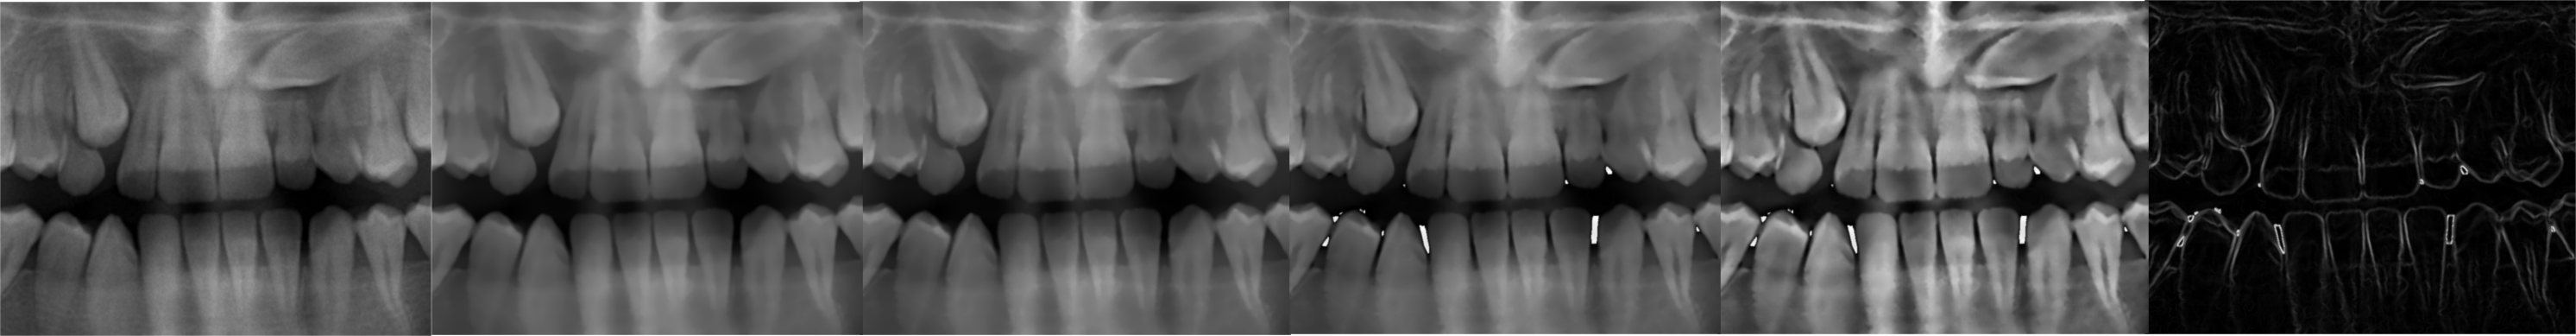
\includegraphics[width=\linewidth]{img/enhancenment}
  \caption{Image after applying the alogorithms}
  \end{figure}
